

\begin{figure}
  \centering
  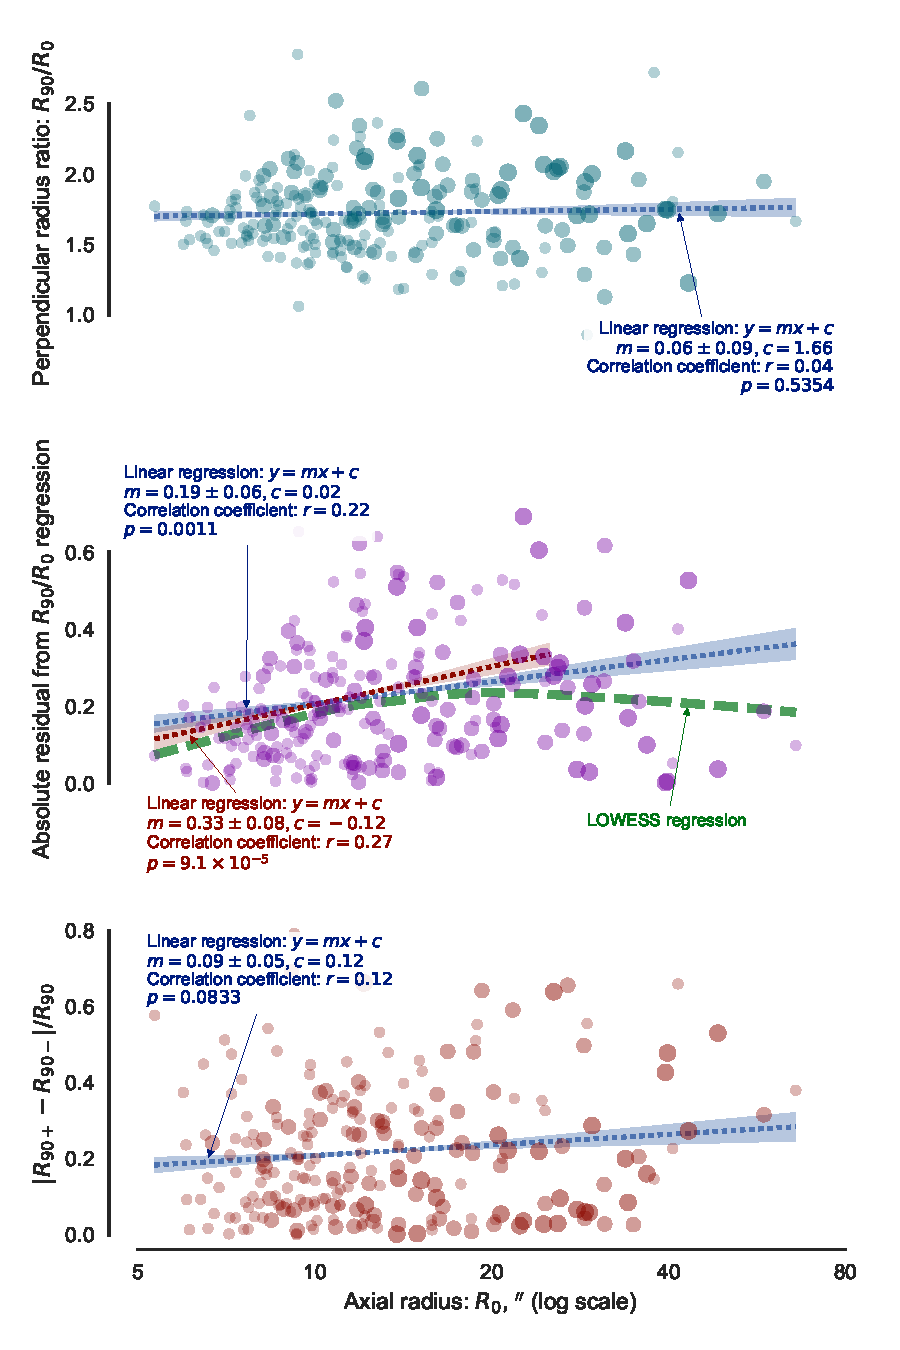
\includegraphics[width=\linewidth]{figs/mipsgal-R90-ratio-versus-R0-heteroscedastic}
  \caption{Regression analysis of bow shock wings shape versus size.
    The top panel shows a linear fit to \(R_{90}/R_0\) versus
    \(\log_{10} R_0\), which is essentially flat and is consistent
    with no correlation between the two quantities.  On the other
    hand, in the central panel, which shows the absolute values of the
    residuals from this fit, it is apparent that the dispersion about
    the average value of the bow shock shape parameter \(R_{90}/R_0\)
    increases with bow shock size.  A linear fit to all the data is
    shown by the blue dotted line, while a locally weighted regression
    (LOWESS; \citealp{Cleveland:1979a, Cleveland:1988a}) is shown by
    the heavy green dashed line.  The negative curvature of the LOWESS
    curve suggests that the slope of the linear fit is a compromise
    between a steeper slope for smaller bow shocks and a flat (or
    negative) slope for the largest bow shocks.  We therefore repeat
    the linear fit, but after excluding sources with \(R_0 > 25''\),
    with results shown by the red dotted line.  The bottom panel shows
    the bow shock wings asymmetry parameter,
    \(|R_{90+} - R_{90-}| / R_{90}\), together with a linear fit.
    Symbol size indicates the star rating of each source, from 3-star
    (smallest) to 5-star (largest).}
  \label{fig:mipsgal-heteroscedastic}
\end{figure}



%%% Local Variables:
%%% mode: latex
%%% TeX-master: "obs-bowshocks"
%%% End:
